\section{Mathematical model for the description of the PMT response}

The goal for using MAPMTs in RICH detectors is to achieve reliable detection of single photons in the Cherenkov light radiation cones. Single photon incident on a PMT face may knock out a single photoelectron from the PMT's photocathode with a certain probability, defined as Quantum Efficiency (QE). The photoelectrons cascade inside the PMT to generate a typical amplified electrical signal at the anode. The amplitude distribution of the single photoelectron (SPE) signals depends on the MAPMT design and high voltage applied, and varies from pixel to pixel. Tests and characterization of multiple MAPMTs include measuring the SPE amplitude distributions for every pixel, finding out the appropriate amplitude thresholds, and determining QE. To achieve this goal we used the methods developed in ~\cite{DEGTIARENKO20171}, expanded to include the new empirical method to take into account the effects of the pixel-to-pixel cross talk in H12700 tubes. The reference ~\cite{DEGTIARENKO20171} describes in detail the mathematical model used to extract and parameterize the SPE distributions from the measurements using the laser test setup. The method allows in principle to describe the SPE functions of essentially any complexity by decomposing them into a sum of Poisson distributions with different averages. For the detailed explanations and the definition of the model parameters please refer to ~\cite{DEGTIARENKO20171}. The list of main parameters includes $\mu$, average number of photoelectrons produced by the laser in a given pixel per one test pulse, and {\it{scale}}, average amplitude of the SPE distribution in pC. Five parameters determine the shape of the SPE distribution, defined as a normalized sum of three Poisson distributions with different average multiplication coefficients applied to the photoelectron on the first dynode of the PMT. Average multiplication on the first cascade ${\nu}$ may be derived from these parameters. ${\sigma}$ parameter describes the Gaussian shape of the pedestal function. ${\xi}$ parameter describes effective cascade multiplication on the second dynode. The combination of 9 parameters describes a single-anode PMT SPE response in an ideal measurement setup with a Gaussian pedestal function. If the pedestal amplitude distribution is not exactly following the Gaussian shape the problem of parameterizing the SPE distribution requires addition of new parameters taking into account the distortion of the pedestal Gaussian. The method was successfully implemented in ~\cite{DEGTIARENKO20171} in the case of small exponential noise contribution to the Gaussian measurement function, see the Eqs. (38-40) in that publication. In the present work we use similar ad hoc approach to parameterize and approximate the contribution of the cross talk signals coming from the neighboring pixels to the SPE amplitude distribution. The model for the process, in agreement with the observations presented in the previous chapter, assumes that a portion of the signal from a neighboring pixel may be randomly added to the amplitude measured in a given pixel under investigation. Such random contribution could in principle depend on the neighbor. It would be impossible to characterize all possible pair combinations. Generally Poissonian shapes of the SPE distribution functions suggests the shape of the cross talk contribution in the form similar to a Poisson distribution scaled to represent the portion of the charge generated in the neighboring pixel and transferred to the pixel studied. A reasonably good approximation of such scaled continuous Poisson-like distribution may take the form 
\begin{equation}
\label{ContPoisson}
 P_c(x;\lambda) = \frac{\lambda^{x} e^{-\lambda}}{\Gamma(x+1)},
\end{equation}
similar to the original Poisson distribution defined for integer x, but expanding the definition to all real $x>0$ values, using the fact that for integer $x = n$ gamma function $\Gamma(x+1) = n!$, and it is continuous in $x$. The function $ P_c(x;\lambda) $ has its average value at $\lambda$ similar to the standard Poisson distribution, and is approximately normalized as a probability distribution. The normalization holds very well at reasonably large $\lambda > \approx 2$, and can be improved in the calculation algorithm. The function of Eq. (\ref{ContPoisson}) may serve as a probability distribution function describing the contribution of an averaged cross talk electron to the SPE distribution
\begin{equation}
\label{fe}
 f_{e}(a;\zeta,\lambda) = \frac{\lambda}{\zeta} P_c \left (\frac{a \lambda}{\zeta};\lambda \right ),
\end{equation}
where $a$ is normalized signal amplitude; $\zeta$ is the scale factor characterizing the average amplitude of an average cross talk signal in units of the $scale$ parameter; and $\lambda$ is the parameter responsible for the Poissonian shape of the cross talk distribution. $\zeta$ must be small compared with $scale$ for the model to work reliably, which is the case for H12700 MAPMTs. Parameter $\lambda$ accommodates the shape of the cross talk function and reflects the effective separation of the cross talk amplitude peak from the pedestal.

One more parameter required for the cross talk model description is $\beta$, which represents the average number of the cross talk electrons per one laser pulse, and is expected to be comparable with $\mu$. Similar to how the measured amplitude distribution during the test is defined by the Poisson sum on the number of photoelectrons $m$ with average $\mu$, the measured cross talk amplitude distribution is defined by the Poisson sum on the number of the cross talk electrons in the neighboring pixels, with average $\beta$: 
\begin{equation}
\label{fCT}
 f_{CT}(a;\beta,\zeta,\lambda) = \sum\limits_{i=1}^{\infty}  \frac{\beta^{i} e^{-\beta}}{i!} \left [ f_{e}(a;\zeta,\lambda) \right ] ^{*i},
\end{equation}
assuming also that similarly to the integer Poisson distributions, the convolution powers of the electron cross talk functions $f_{e}$ may be explicitly calculated as  
\begin{equation}
\label{fe_cp}
 \left [ f_{e}(a;\zeta,\lambda) \right ] ^{*i} = \frac{\lambda}{\zeta} P_c \left (\frac{a \lambda}{\zeta};i\lambda \right ).
\end{equation}

The approximation implemented in this work assumes that the amplitude of the cross talk contribution is relatively small compared with the average SPE amplitude and may be considered an addition to the Gaussian measurement function, similar to how it was implemented in Eq.~(39) of ~\cite{DEGTIARENKO20171}. The Gaussian form $G(a,n;\sigma_{\mathrm{eff}})$ in the main model calculation Eq.~(36) of ~\cite{DEGTIARENKO20171} can be substituted with the corrected measurement function  
\begin{equation}
  \label{EMGform}
\exp(-\beta) \times G(a,n;\sigma_{\mathrm{eff}}) + f_{CT}(a;\beta,\zeta,\lambda) .
\end{equation}

The technique is illustrated in Fig.~\ref{fig:Model} showing an example of an SPE function for the distribution of the test events on the normalized measured charge $a$, with $a=1$ corresponding to the average charge collected from one photoelectron. The series of lines marked as $m = 1, 2, 3$ correspond to the charge distributions in the events with corresponding number of photoelectrons, assuming the average number of photoelectrons in test event is $\mu = 0.2$. Red distribution corresponds to the pedestal measurement function $G$ with the added cross talk correction. Regions in this distribution marked with $\mathrm{N_{cte}=0, 1, 2}$ correspond to the original Gaussian pedestal function and the contributions from one and two cross talk electrons. The parameters are selected for better visibility of the cross talk effects, with $\beta$ equal to $\mu$, $\zeta$ equal to 10\% of the $scale$ parameter, and $\lambda = 5$ to make the cross talk Poisson peak more visible.  

The fitting procedure from ~\cite{DEGTIARENKO20171} was modified to include the new three parameters in the FORTRAN routine describing the measured test spectra, bringing the total number of parameters to 12. The algorithm for the multiparametric minimization was adjusted correspondingly to provide stability. The experimental verification of the fit stability and reproduceability of the results was performed using multiple measurements of the same MAPMTs in the different slots in the test setup and comparing the results. Overall confidence was also assured by extracting parameters for each MAPMT in several test conditions, varying the high voltage and the illumination conditions, and verifying the consistency in the values of the extracted parameters. 

\begin{figure}[t]
	\centering
	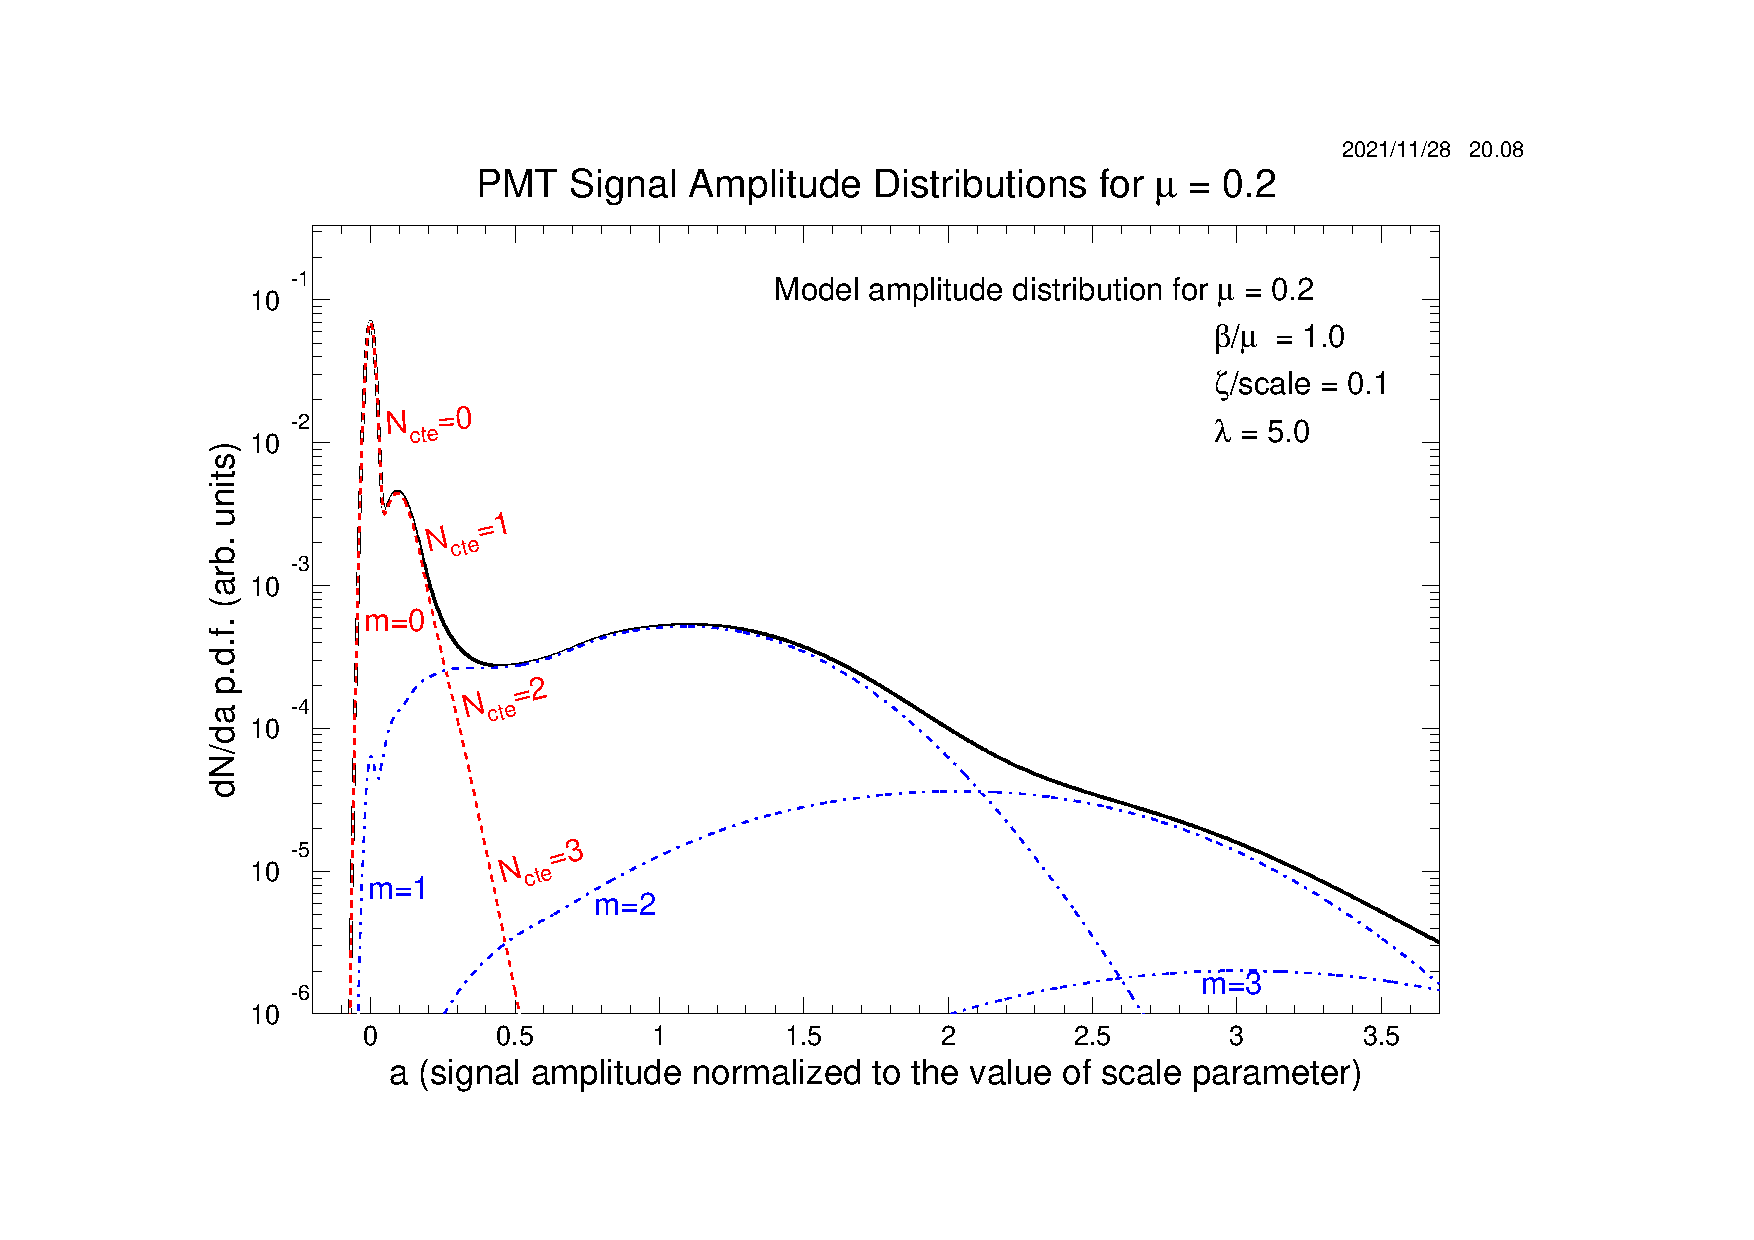
\includegraphics[trim=90 60 110 100, clip, width=\linewidth]{figures/model.pdf}
	\caption{Model signal charge distribution (black line) illustrating the parameterization for the cross talk effects. Red trace ($m = 0$) corresponds to the pedestal measurement function with the additional cross talk contribution, violet lines ($m = 1, 2, 3$) show contributions from events with the number of photoelectrons 1, 2, and 3, with their relative probability corresponding to the Poisson distribution with average $\mu = 0.2$  }
	\label{fig:Model}
\end{figure}
